\documentclass{standalone}
\usepackage{tikz}
\usetikzlibrary{patterns, positioning}
\usepackage[sfdefault]{ClearSans} %% option 'sfdefault' activates Clear Sans as the default text font
\usepackage[T1]{fontenc}

\begin{document}
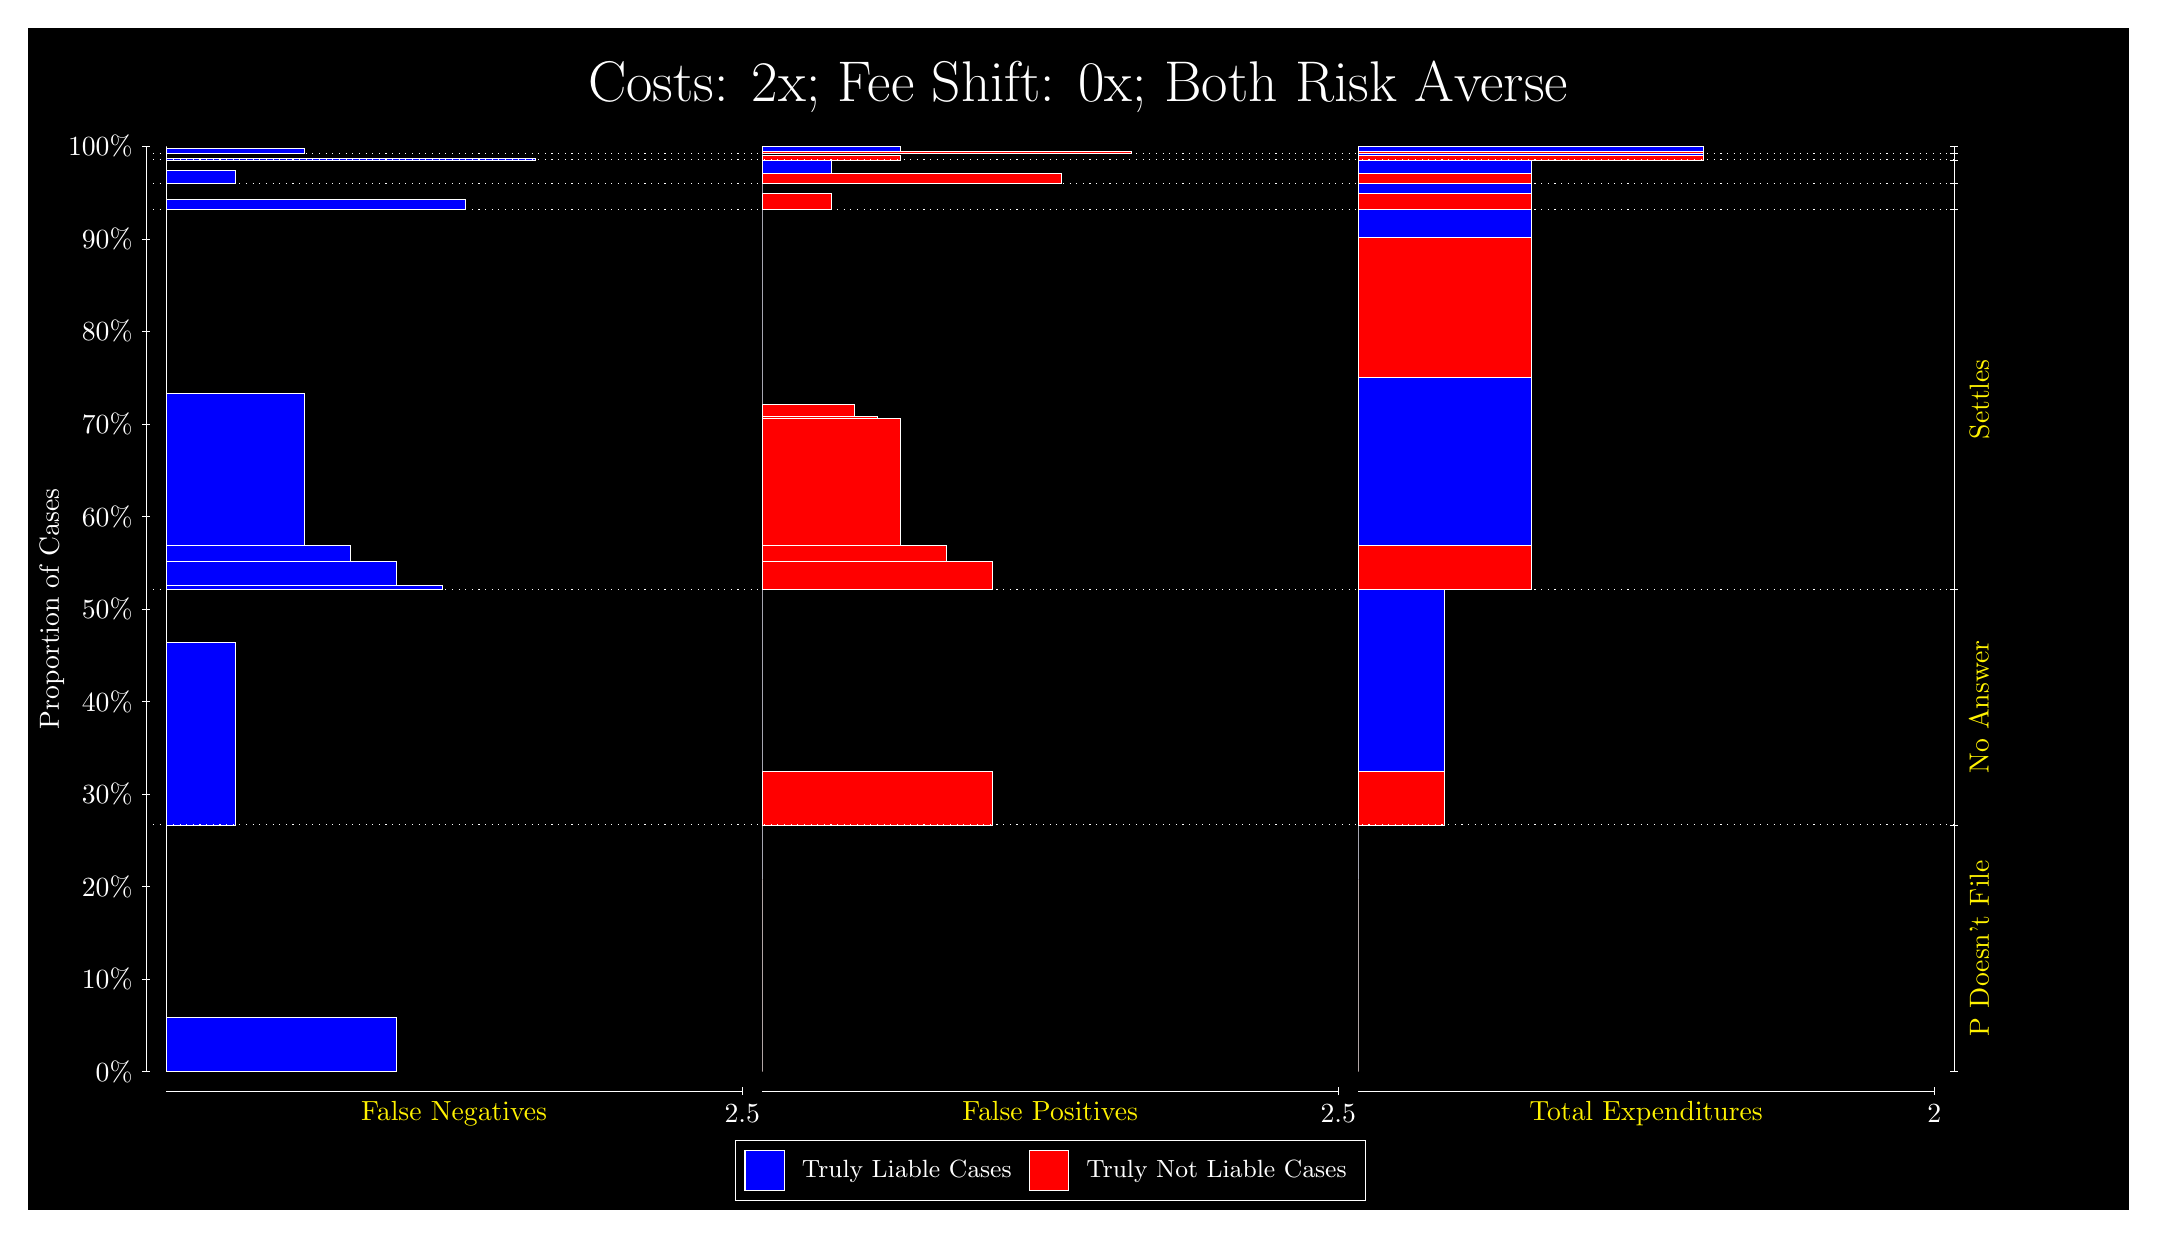
\begin{tikzpicture}
\draw[fill=black] (0,0) rectangle (26.667,15);
\draw[text=white] (0,13.5) rectangle (26.667,15) node[midway] {\huge Costs: 2x; Fee Shift: 0x; Both Risk Averse};
\draw[white, very thin] (1.5,1.75) -- (1.5,13.5);
\node[rotate=90, text=white, anchor=center] at (0.3, 7.625) {Proportion of Cases};
\draw[white, very thin] (1.45,1.75) -- (1.55,1.75);
\node[text=white, anchor=east] at (1.45, 1.75) {0\%};
\draw[white, very thin] (1.45,2.925) -- (1.55,2.925);
\node[text=white, anchor=east] at (1.45, 2.925) {10\%};
\draw[white, very thin] (1.45,4.1) -- (1.55,4.1);
\node[text=white, anchor=east] at (1.45, 4.1) {20\%};
\draw[white, very thin] (1.45,5.275) -- (1.55,5.275);
\node[text=white, anchor=east] at (1.45, 5.275) {30\%};
\draw[white, very thin] (1.45,6.45) -- (1.55,6.45);
\node[text=white, anchor=east] at (1.45, 6.45) {40\%};
\draw[white, very thin] (1.45,7.625) -- (1.55,7.625);
\node[text=white, anchor=east] at (1.45, 7.625) {50\%};
\draw[white, very thin] (1.45,8.8) -- (1.55,8.8);
\node[text=white, anchor=east] at (1.45, 8.8) {60\%};
\draw[white, very thin] (1.45,9.975) -- (1.55,9.975);
\node[text=white, anchor=east] at (1.45, 9.975) {70\%};
\draw[white, very thin] (1.45,11.15) -- (1.55,11.15);
\node[text=white, anchor=east] at (1.45, 11.15) {80\%};
\draw[white, very thin] (1.45,12.325) -- (1.55,12.325);
\node[text=white, anchor=east] at (1.45, 12.325) {90\%};
\draw[white, very thin] (1.45,13.5) -- (1.55,13.5);
\node[text=white, anchor=east] at (1.45, 13.5) {100\%};

\draw[white, very thin] (24.457,1.75) -- (24.457,13.5);
\draw[white, very thin] (24.407,1.75) -- (24.507,1.75);
\node[anchor=west] at (24.407, 1.75) {};
\draw[white, very thin] (24.407,4.883) -- (24.507,4.883);
\node[anchor=west] at (24.407, 4.883) {};
\draw[white, very thin] (24.407,7.8754) -- (24.507,7.8754);
\node[anchor=west] at (24.407, 7.8754) {};
\draw[white, very thin] (24.407,12.701) -- (24.507,12.701);
\node[anchor=west] at (24.407, 12.701) {};
\draw[white, very thin] (24.407,13.025) -- (24.507,13.025);
\node[anchor=west] at (24.407, 13.025) {};
\draw[white, very thin] (24.407,13.327) -- (24.507,13.327);
\node[anchor=west] at (24.407, 13.327) {};
\draw[white, very thin] (24.407,13.414) -- (24.507,13.414);
\node[anchor=west] at (24.407, 13.414) {};
\draw[white, very thin] (24.407,13.5) -- (24.507,13.5);
\node[anchor=west] at (24.407, 13.5) {};

\draw[white, very thin, fill=blue] (1.75,1.75) rectangle (4.6775,2.4412);
\draw[white, very thin, fill=red] (1.75,2.4412) rectangle (1.75,4.883);
\draw[white, very thin, fill=blue] (1.75,4.883) rectangle (2.6283,7.1967);
\draw[white, very thin, fill=red] (1.75,7.1967) rectangle (1.75,7.8754);
\draw[white, very thin, fill=blue] (1.75,7.8754) rectangle (5.2631,7.9207);
\draw[white, very thin, fill=blue] (1.75,7.9207) rectangle (4.9703,7.9298);
\draw[white, very thin, fill=blue] (1.75,7.9298) rectangle (4.6775,8.2251);
\draw[white, very thin, fill=blue] (1.75,8.2251) rectangle (4.092,8.428);
\draw[white, very thin, fill=blue] (1.75,8.428) rectangle (3.5065,10.358);
\draw[white, very thin, fill=red] (1.75,10.358) rectangle (1.75,12.701);
\draw[white, very thin, fill=blue] (1.75,12.701) rectangle (5.5558,12.828);
\draw[white, very thin, fill=red] (1.75,12.828) rectangle (1.75,13.025);
\draw[white, very thin, fill=blue] (1.75,13.025) rectangle (2.6283,13.199);
\draw[white, very thin, fill=red] (1.75,13.199) rectangle (1.75,13.327);
\draw[white, very thin, fill=blue] (1.75,13.327) rectangle (6.4341,13.354);
\draw[white, very thin, fill=red] (1.75,13.354) rectangle (1.75,13.414);
\draw[white, very thin, fill=blue] (1.75,13.414) rectangle (3.5065,13.473);
\draw[white, very thin, fill=red] (1.75,13.473) rectangle (1.75,13.5);
\draw[white, very thin, fill=red] (9.3189,1.75) rectangle (9.3189,4.1919);
\draw[white, very thin, fill=blue] (9.3189,4.1919) rectangle (9.3189,4.883);
\draw[white, very thin, fill=red] (9.3189,4.883) rectangle (12.246,5.5617);
\draw[white, very thin, fill=blue] (9.3189,5.5617) rectangle (9.3189,7.8754);
\draw[white, very thin, fill=red] (9.3189,7.8754) rectangle (12.246,8.2326);
\draw[white, very thin, fill=red] (9.3189,8.2326) rectangle (11.661,8.4355);
\draw[white, very thin, fill=red] (9.3189,8.4355) rectangle (11.075,10.04);
\draw[white, very thin, fill=red] (9.3189,10.04) rectangle (10.783,10.066);
\draw[white, very thin, fill=red] (9.3189,10.066) rectangle (10.49,10.218);
\draw[white, very thin, fill=blue] (9.3189,10.218) rectangle (9.3189,12.701);
\draw[white, very thin, fill=red] (9.3189,12.701) rectangle (10.197,12.898);
\draw[white, very thin, fill=blue] (9.3189,12.898) rectangle (9.3189,13.025);
\draw[white, very thin, fill=red] (9.3189,13.025) rectangle (13.125,13.153);
\draw[white, very thin, fill=blue] (9.3189,13.153) rectangle (10.197,13.327);
\draw[white, very thin, fill=red] (9.3189,13.327) rectangle (11.075,13.387);
\draw[white, very thin, fill=blue] (9.3189,13.387) rectangle (9.3189,13.414);
\draw[white, very thin, fill=red] (9.3189,13.414) rectangle (14.003,13.441);
\draw[white, very thin, fill=blue] (9.3189,13.441) rectangle (11.075,13.5);
\draw[white, very thin, fill=red] (16.888,1.75) rectangle (16.888,4.1919);
\draw[white, very thin, fill=blue] (16.888,4.1919) rectangle (16.888,4.883);
\draw[white, very thin, fill=red] (16.888,4.883) rectangle (17.986,5.5617);
\draw[white, very thin, fill=blue] (16.888,5.5617) rectangle (17.986,7.8754);
\draw[white, very thin, fill=red] (16.888,7.8754) rectangle (19.083,8.4355);
\draw[white, very thin, fill=blue] (16.888,8.4355) rectangle (19.083,10.569);
\draw[white, very thin, fill=red] (16.888,10.569) rectangle (19.083,12.351);
\draw[white, very thin, fill=blue] (16.888,12.351) rectangle (19.083,12.701);
\draw[white, very thin, fill=red] (16.888,12.701) rectangle (19.083,12.898);
\draw[white, very thin, fill=blue] (16.888,12.898) rectangle (19.083,13.025);
\draw[white, very thin, fill=red] (16.888,13.025) rectangle (19.083,13.153);
\draw[white, very thin, fill=blue] (16.888,13.153) rectangle (19.083,13.327);
\draw[white, very thin, fill=red] (16.888,13.327) rectangle (21.279,13.387);
\draw[white, very thin, fill=blue] (16.888,13.387) rectangle (21.279,13.414);
\draw[white, very thin, fill=red] (16.888,13.414) rectangle (21.279,13.441);
\draw[white, very thin, fill=blue] (16.888,13.441) rectangle (21.279,13.5);
\draw[white, dotted] (1.5,4.883) -- (24.457,4.883);
\draw[white, dotted] (1.5,7.8754) -- (24.457,7.8754);
\draw[white, dotted] (1.5,12.701) -- (24.457,12.701);
\draw[white, dotted] (1.5,13.025) -- (24.457,13.025);
\draw[white, dotted] (1.5,13.327) -- (24.457,13.327);
\draw[white, dotted] (1.5,13.414) -- (24.457,13.414);
\draw[white, very thin] (1.75,1.5) -- (9.0689,1.5);
\node[text=yellow, anchor=north] at (5.4094, 1.5) {False Negatives};
\draw[white, very thin] (9.0689,1.45) -- (9.0689,1.55);
\node[text=white, anchor=north] at (9.0689, 1.45) {2.5};

\draw[white, very thin] (9.3189,1.5) -- (16.638,1.5);
\node[text=yellow, anchor=north] at (12.978, 1.5) {False Positives};
\draw[white, very thin] (16.638,1.45) -- (16.638,1.55);
\node[text=white, anchor=north] at (16.638, 1.45) {2.5};

\draw[white, very thin] (16.888,1.5) -- (24.207,1.5);
\node[text=yellow, anchor=north] at (20.547, 1.5) {Total Expenditures};
\draw[white, very thin] (24.207,1.45) -- (24.207,1.55);
\node[text=white, anchor=north] at (24.207, 1.45) {2};

\node[text=yellow, centered, rotate=90] at (24.777, 3.3165) {P Doesn't File};
\node[text=yellow, centered, rotate=90] at (24.777, 6.3792) {No Answer};
\node[text=yellow, centered, rotate=90] at (24.777, 10.288) {Settles};





\draw (12.978300999999998,1.5) node[draw=none] (baseCoordinate) {};
\begin{scope}[align=center]
        \matrix[scale=0.5, draw=white, below=0.5cm of baseCoordinate, nodes={draw}, column sep=0.1cm]{
            \node[rectangle, draw, minimum width=0.5cm, minimum height=0.5cm, fill=blue] {}; &
            \node[draw=none, font=\small, text=white] (B) {Truly Liable Cases}; &
            \node[rectangle, draw, minimum width=0.5cm, minimum height=0.5cm, fill=red] {}; &
            \node[draw=none, font=\small, text=white] (B) {Truly Not Liable Cases}; \\
            };
\end{scope}

\end{tikzpicture}
\end{document}